\documentclass[]{standalone}
%\usepackage{mathptmx}
%\renewcommand{\familydefault}{\rmdefault}
\usepackage[T1]{fontenc}
\usepackage[latin9]{inputenc}
\usepackage{siunitx}
\usepackage{array}
\usepackage{amsmath}
\usepackage{ifthen}
\usepackage{pgfplots}
\usepackage{pgfmath}
\pgfplotsset{compat=1.14}
\usepackage{titling, graphicx}
\usepackage{tikz}
\usepackage{upgreek}
\usepackage{amsmath,amsthm}
\usepackage{strtikz}
\usetikzlibrary{shapes,arrows.meta,intersections,graphs,graphs.standard}
\usetikzlibrary{math,fit}
\usetikzlibrary{calc,intersections,through,backgrounds,decorations.pathmorphing}


\begin{document}
\begin{tikzpicture}
\def \framelinethickness {1pt}
\def \springlinethickness {0.5pt}
\def \springradius {0.0005cm}
\def \springcycle {4}
\def \springradcoeff {0.5}
\rotspring[startx = 0cm,
  starty = 0cm,
  rotation = 0,
  start rigid length = 2cm,
  end rigid length = 1.5cm,
  rotational spring diameter = \springradius,
  rotational spring cycle number = \springcycle,
  text = $k_\theta$,
  text location = above,
  text location offset = 2pt,
  rigid thickness = \framelinethickness,
  spring thickness = \springlinethickness,
  spring direction mode = 1,
  radius coefficient = \springradcoeff,
  rigid left text = {$L_1=0$},
  rigid right text = {$L_2=0$},
  rigid text offset = -2pt]
\end{tikzpicture}
\end{document}